\documentclass[a4paper, UKenglish, cleveref, autoref, thm-restate, colorlinks]{lipics-v2021}

\usepackage{amsmath}
\usepackage{prooftree}
\usepackage{tikz}

\usetikzlibrary{patterns}

\bibliographystyle{plainurl}

\newcommand{\eps}[1]{\epsilon{#1}.}
\newcommand{\fall}[1]{\forall{#1}.}
\newcommand{\lam}[1]{\lambda{#1}.}
\newcommand{\xsts}[1]{\exists{#1}.}

\title{All watched over by machines of loving grace}
\titlerunning{Supervisionary system description}

\begin{CCSXML}
<ccs2012>
   <concept>
       <concept_id>10003752.10003790.10003800</concept_id>
       <concept_desc>Theory of computation~Higher order logic</concept_desc>
       <concept_significance>300</concept_significance>
       </concept>
   <concept>
       <concept_id>10003752.10003790.10003794</concept_id>
       <concept_desc>Theory of computation~Automated reasoning</concept_desc>
       <concept_significance>500</concept_significance>
       </concept>
   <concept>
       <concept_id>10003752.10003790.10002990</concept_id>
       <concept_desc>Theory of computation~Logic and verification</concept_desc>
       <concept_significance>500</concept_significance>
       </concept>
   <concept>
       <concept_id>10011007.10010940.10010941.10010949</concept_id>
       <concept_desc>Software and its engineering~Operating systems</concept_desc>
       <concept_significance>300</concept_significance>
       </concept>
 </ccs2012>
\end{CCSXML}

\ccsdesc[300]{Theory of computation~Higher order logic}
\ccsdesc[500]{Theory of computation~Automated reasoning}
\ccsdesc[500]{Theory of computation~Logic and verification}
\ccsdesc[300]{Software and its engineering~Operating systems}

\keywords{Proof assistant design, operating systems, HOL, LCF, Supervisionary, system description, capabilities}

\author{Dominic P. Mulligan}{Automated Reasoning Group, Amazon Web Services, Cambridge, United Kingdom\footnote{All work done whilst employed within the Systems Research Group, Arm Research, Cambridge} \and \url{www.dominic-mulligan.co.uk}}{dominic.p.mulligan@gmail.com}{}{}
\authorrunning{Dominic P. Mulligan}

\Copyright{Dominic P. Mulligan}

\acknowledgements{}

\begin{document}

\maketitle

\begin{abstract}
Modern operating systems are typically built around a trusted system component called the \emph{kernel} which amongst other things is charged with enforcing system-wide security policies.
Crucially, this component must be kept isolated from untrusted software at all times, which is facilitated by exploiting machine-oriented notions of separation: private memories, privilege levels, and similar.

Modern proof-assistants are typically built around a trusted system component called the \emph{kernel} which is charged with enforcing system-wide soundness.
Crucially, this component must be kept isolated from untrusted automation at all times, which is facilitated by exploiting programming-language notions of separation: module-private data structures, type-abstraction, and similar.

Whilst markedly different in purpose, in some essential ways operating system and proof-assistant kernels are tasked with the same job, namely enforcing system-wide invariants in the face of unbridled interaction with untrusted code.  Yet the mechanisms through which the two types of kernel protect themselves are significantly different.
In this paper, we introduce \emph{Supervisionary}, the kernel of a prototype programmable proof-checking system for Gordon's HOL that is organised in a manner more reminiscent of operating systems than typical LCF-style proof-checkers.
Supervisionary implements a kernel that executes at a relative level of privilege compared to untrusted automation, with trusted and untrusted system components communicating across a limited system call boundary to indirectly manipulate kernel objects managed by the Supervisionary kernel denoted by handles.

Unusually, Supervisionary has no ``metalanguage'' in the LCF sense, as the language used to implement the kernel, and the language used to implement automation, need not be the same.
\emph{Any} programming language can be used to implement automation for Supervisionary, providing the resulting binary respects the Supervisionary kernel calling convention and binary interface, with no risk to system soundness.
Further, we observe that Supervisionary allows arbitrary programming languages to be endowed with facilities for proof-checking.
Indeed, the handles that Supervisionary uses to reference kernel objects under its management may be thought of as a form of \emph{capability}, in the computer security sense.
Moreover, these capabilities are extremely expressive, essentially capturing the full expressive power of HOL, and can potentially be used to enforce fine-grained correctness and security properties of programs at runtime.
\end{abstract}

\section{Introduction}
\label{sect.introduction}

This paper studies the intersection of operating system design and implementations of the foundations of mathematics.
Research into the confluence of these two topics is, admittedly, a rather moribund affair at the moment.
Nevertheless, with this paper we hope to convince the reader that probing the intersection of these two areas is potentially very interesting by introducing \emph{Supervisionary}, a programmable proof-checking system for Gordon's HOL.
This system has a novel system design, with some interesting properties, and moreover some interesting consequences.
First, however, we begin with a scene-setting overview of common principles in operating system design and implementation.

\subsection{On operating systems}

\begin{figure}
\tikzset{every picture/.style={line width=0.75pt}} %set default line width to 0.75pt        
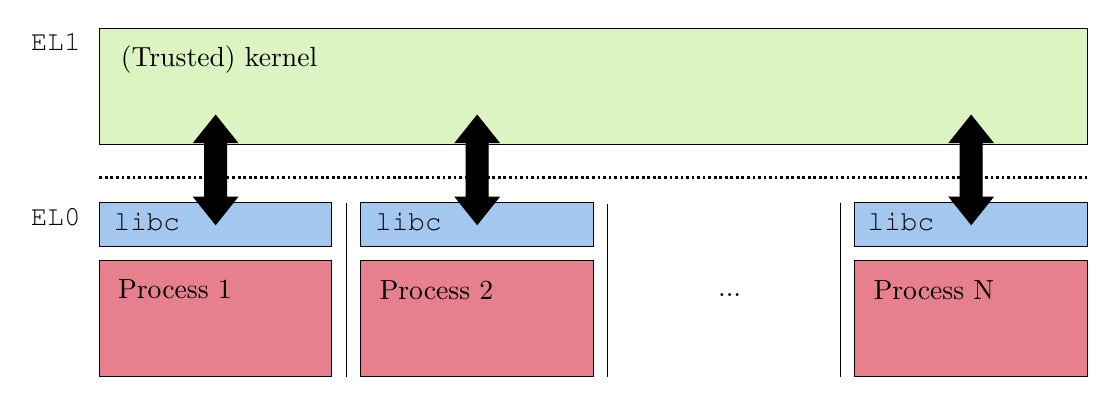
\begin{tikzpicture}[x=0.75pt,y=0.75pt,yscale=-0.7,xscale=0.7]
%uncomment if require: \path (0,300); %set diagram left start at 0, and has height of 300

%Straight Lines [id:da0238858095373361] 
\draw [line width=1]  [dash pattern={on 1pt off 1pt}]  (10,133) -- (690,133) ;
%Shape: Rectangle [id:dp18633003951104476] 
\draw  [fill={rgb, 255:red, 184; green, 233; blue, 134 }  ,fill opacity=0.5 ] (10,30) -- (690,30) -- (690,110) -- (10,110) -- cycle ;
%Straight Lines [id:da8836005156472156] 
\draw    (180,150) -- (180,270) ;
%Straight Lines [id:da0871105771687758] 
\draw    (360,151) -- (360,270) ;
%Straight Lines [id:da47486673087950704] 
\draw    (520,150) -- (520,270) ;
%Flowchart: Process [id:dp5014112861074582] 
\draw  [fill={rgb, 255:red, 208; green, 2; blue, 27 }  ,fill opacity=0.5 ] (10,190) -- (170,190) -- (170,270) -- (10,270) -- cycle ;
%Flowchart: Process [id:dp5474401833590941] 
\draw  [fill={rgb, 255:red, 208; green, 2; blue, 27 }  ,fill opacity=0.5 ] (190,190) -- (350,190) -- (350,270) -- (190,270) -- cycle ;
%Flowchart: Process [id:dp05943677937308278] 
\draw  [fill={rgb, 255:red, 208; green, 2; blue, 27 }  ,fill opacity=0.5 ] (530,190) -- (690,190) -- (690,270) -- (530,270) -- cycle ;
%Flowchart: Process [id:dp22719106375428721] 
\draw  [fill={rgb, 255:red, 74; green, 144; blue, 226 }  ,fill opacity=0.5 ] (10,150) -- (170,150) -- (170,180) -- (10,180) -- cycle ;
%Flowchart: Process [id:dp418634561741007] 
\draw  [fill={rgb, 255:red, 74; green, 144; blue, 226 }  ,fill opacity=0.5 ] (190,150) -- (350,150) -- (350,180) -- (190,180) -- cycle ;
%Flowchart: Process [id:dp5808126324898445] 
\draw  [fill={rgb, 255:red, 74; green, 144; blue, 226 }  ,fill opacity=0.5 ] (530,150) -- (690,150) -- (690,180) -- (530,180) -- cycle ;
%Left Right Arrow [id:dp18252152506193997] 
\draw  [fill={rgb, 255:red, 0; green, 0; blue, 0 }  ,fill opacity=1 ] (90,90) -- (105,108.75) -- (97.5,108.75) -- (97.5,146.25) -- (105,146.25) -- (90,165) -- (75,146.25) -- (82.5,146.25) -- (82.5,108.75) -- (75,108.75) -- cycle ;
%Left Right Arrow [id:dp937447124008122] 
\draw  [fill={rgb, 255:red, 0; green, 0; blue, 0 }  ,fill opacity=1 ] (270,90) -- (285,108.75) -- (277.5,108.75) -- (277.5,146.25) -- (285,146.25) -- (270,165) -- (255,146.25) -- (262.5,146.25) -- (262.5,108.75) -- (255,108.75) -- cycle ;
%Left Right Arrow [id:dp43564214029042536] 
\draw  [fill={rgb, 255:red, 0; green, 0; blue, 0 }  ,fill opacity=1 ] (610,90) -- (625,108.75) -- (617.5,108.75) -- (617.5,146.25) -- (625,146.25) -- (610,165) -- (595,146.25) -- (602.5,146.25) -- (602.5,108.75) -- (595,108.75) -- cycle ;

% Text Node
\draw (23,40) node [anchor=north west][inner sep=0.75pt]   [align=left] {{\fontfamily{rm}\selectfont (Trusted) kernel}};
% Text Node
\draw (434,211) node [anchor=north west][inner sep=0.75pt]   [align=left] {{\fontfamily{rm}\selectfont ...}};
% Text Node
\draw (18,155) node [anchor=north west][inner sep=0.75pt]   [align=left] {{\fontfamily{pcr}\selectfont libc}};
% Text Node
\draw (198,155) node [anchor=north west][inner sep=0.75pt]   [align=left] {{\fontfamily{pcr}\selectfont libc}};
% Text Node
\draw (537,155) node [anchor=north west][inner sep=0.75pt]   [align=left] {{\fontfamily{pcr}\selectfont libc}};
% Text Node
\draw (21,201) node [anchor=north west][inner sep=0.75pt]   [align=left] {{\fontfamily{rm}\selectfont Process 1}};
% Text Node
\draw (201,202) node [anchor=north west][inner sep=0.75pt]   [align=left] {{\fontfamily{rm}\selectfont Process 2}};
% Text Node
\draw (541,202) node [anchor=north west][inner sep=0.75pt]   [align=left] {{\fontfamily{rm}\selectfont Process N}};
% Text Node
\draw (-39,32) node [anchor=north west][inner sep=0.75pt]   [align=left] {{\fontfamily{pcr}\selectfont EL1}};
% Text Node
\draw (-39,152) node [anchor=north west][inner sep=0.75pt]   [align=left] {{\fontfamily{pcr}\selectfont EL0}};
\end{tikzpicture}
\caption{A schematic of the typical system organization of a commodity operating system and its associated user-space.
The kernel (in green) executes at a relative level of privilege, enforced by hardware, compared to processes executing in user-space (red)---we follow the Arm convention and show the kernel executing at \texttt{EL1} and user-space at \texttt{EL0}.
The two communicate across a system call boundary (dashed line) using system calls (black arrows).
User-space programs are typically written making use of an abstraction library, such as \texttt{libc} (blue), to abstract over this kernel interface.}
\label{fig.operating-system.schematic}
\end{figure}

Most commodity operating systems---that is, Microsoft Windows and Unix-derivatives\footnote{\emph{Commodity} here is used to guard against pedantic quibbling over research operating system designs---like exokernels and other oddities---which arguably do not fit this pattern}---fit a common pattern and are architected around a relatively self-contained, trusted component typically called the system \emph{kernel}.

The kernel is the sole component that can interface unfettered with all system resources, including devices and other system hardware.
Untrusted user-space applications make use of kernel interfaces in order to make use of a device or any other system resource managed by the kernel.
As a result, the kernel is essentially a ``pinch point'' for gating access to system resources.
The kernel also introduces a process abstraction in user-space and is responsible for ensuring the confidentiality and integrity of processes from other, concurrently executing processes.
The kernel is therefore \emph{the} key component responsible for enforcing system-wide security policies, and essentially forms the ``root of all trust'' within a computing system.
It is therefore imperative that the kernel is itself isolated sufficiently from user-space software at all times, lest this role be undermined by a malefactor.

The kernel self-isolates by entering into a grand conspiracy with its host hardware.
In support of this conspiracy, mainstream microprocessors have, over the years, accreted a variety of now-familiar security features that an operating system kernel can use to defend itself from prying or interference.
These include \emph{exception levels} or \emph{privilege rings}---as they are variously called, depending on the instruction set architecture---which introduce a notion of \emph{privilege} into the system.
Here, software executing at higher-privilege---in our case, an operating system kernel\footnote{Note that ``Cloud hosting'' as a viable business proposition essentially rests on this trick being repeated again, with a hypervisor sat in a position of privilege compared to an operating system kernel---executing out of an even higher exception level---and enforcing separation betwixt operating system instances.}---gains permission to program sensitive system registers, controlling how the system operates.
Moreover, software executing at a higher-level of privilege can ``peer in'' and potentially modify the runtime state of software executing at a relatively lower-level of privilege, reading data from, or writing data to, a buffer within the memory space of an untrusted user-space process, for example.
In this sense, a kernel can ``supervise'' or ``watch over'' untrusted user-space---essentially the inspiration for the, possibly now archaic, alternative phrasing for an operating system kernel: \emph{supervisor}.

Moreover, modern microprocessors also provide a form of memory management built around page tables.
These data structures have a dual role: primarily, they are used for the virtualisation of system memory via address translation, granting user-space software the illusion that it owns the entire physical address space of the machine, by presenting a virtual address space to user-space programs.
Essentially, address translation induces a notion of \emph{ownership} of pages of physical memory within the system, with a page of physical memory ``owned'' by a principal (either the operating system, or a user-space process) if it is ``mapped in'' to that principal's address space.
Moreover, page tables are also used for storing the attributes of pages of memory, including read-write-execute permissions.
By correctly initialising and managing these tables the kernel is able to keep its own code and data structures isolated---in a kernel-private memory area---that only it can access, safe from prying or interference by untrusted user-space.
As a result, for systems software on modern machines, isolation is enforced by a mix of low-level machine mechanisms: separate address spaces, private memory regions, and machine-enforced privilege checks on executing software.

To make itself useful, the kernel exposes a limited interface, used by user-space to request intercession by the kernel on its behalf---for example by granting user-space access to some device, the filesystem, a socket, or some other system resource under kernel management.
Dealing in generalities, to do this, the kernel exposes a suite of \emph{system calls} which can be invoked by user-space programs with dedicated machine instructions provided by the microprocessor---see Figure~\ref{fig.operating-system.schematic} for a diagrammatic schematic, for example.
On Arm platforms, with which the author is most familiar, these instructions induce a type of processor exception, inducing a \emph{context switch} which flips the flow of control into the kernel's system call handler before eventually returning the flow of control back to the calling user-space program.
From user-space's point-of-view, system calls therefore have the appearance and effect of very CISC-like machine instructions, with the operating system kernel essentially presenting itself to user-space as ``silicon by other means'', extending the user-space fragment of the instruction set architecture of the microprocessor with new instructions.

Note that for this two-way dance to work, user-space and the kernel must work together by adopting a series of joint conventions.
These include a \emph{calling convention} describing how arguments and results are passed back-and-forth across the system call interface, and a \emph{binary interface} detailing how system calls are identified, how errors are reported back to user-space, and other miscellanea.
To help programmers adhere to these conventions, the operating system typically provides an abstraction layer to user-space, which on Unix variants typically takes the form of the system's C library, \texttt{libc}.
Note that this is generally just a convenience, and user-space software can always invoke system calls directly if wanted by invoking the correct machine instruction and adhering to the appropriate calling convention.\footnote{This is the case on Linux, though does not hold universally on all Unix derivatives.  For example Apple's MacOS and some BSD Unix variants generally consider the programming interface of the system C library as the interface of the kernel, proper, in some cases preventing any user-space code other than the system's \texttt{libc} library from invoking system calls directly, as a security mechanism.}

However, crucially, it is \emph{generally} not the case that the operating system kernel and untrusted user-space applications need be written in the same programming language for this all to work.
In particular, whilst most operating system kernels are written in C, or a C-language derivative, user-space programs can be written in a variety of languages, and are also commonly composed of multiple libraries, written in different programming languages, linked together.
Despite this, all are able to make use of system resources exposed by the kernel's system call interface by ensuring that they adhere to the calling convention and binary interface expected by the kernel.
In this respect, for commodity operating systems, the C-language may have prominence as the favoured language of system implementation, but by-and-large it is not \emph{special} or given an unduly prominent status by the kernel itself.

\subsection{On programmable proof-checkers}

\begin{figure}
\tikzset{every picture/.style={line width=0.75pt}} %set default line width to 0.75pt        
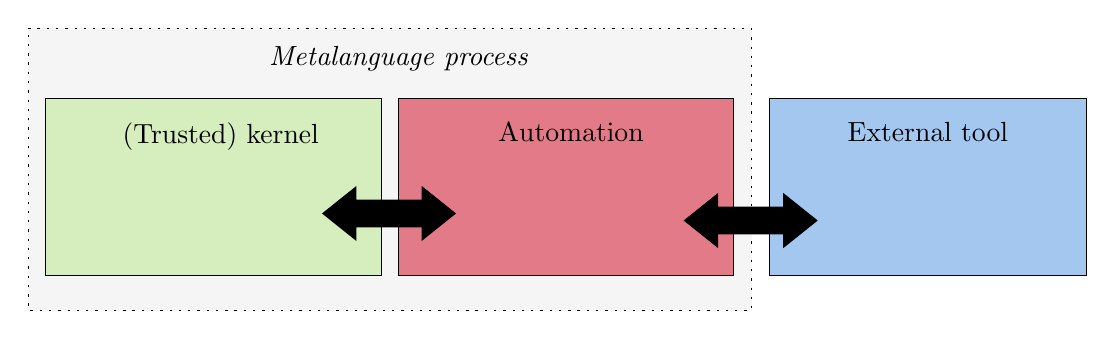
\begin{tikzpicture}[x=0.75pt,y=0.75pt,yscale=-0.85,xscale=0.85]
%uncomment if require: \path (0,300); %set diagram left start at 0, and has height of 300

%Shape: Rectangle [id:dp5145169571980753] 
\draw  [fill={rgb, 255:red, 155; green, 155; blue, 155 }  ,fill opacity=0.1 ][dash pattern={on 0.84pt off 2.51pt}] (10,10) -- (420,10) -- (420,170) -- (10,170) -- cycle ;
%Shape: Rectangle [id:dp7336028259076729] 
\draw  [fill={rgb, 255:red, 184; green, 233; blue, 134 }  ,fill opacity=0.5 ] (20,50) -- (210,50) -- (210,150) -- (20,150) -- cycle ;
%Shape: Rectangle [id:dp32707998554431983] 
\draw  [fill={rgb, 255:red, 208; green, 2; blue, 27 }  ,fill opacity=0.5 ] (220,50) -- (410,50) -- (410,150) -- (220,150) -- cycle ;
%Shape: Rectangle [id:dp3433596839522859] 
\draw  [fill={rgb, 255:red, 74; green, 144; blue, 226 }  ,fill opacity=0.5 ] (430,50) -- (610,50) -- (610,150) -- (430,150) -- cycle ;
%Left Right Arrow [id:dp2058390242799486] 
\draw  [fill={rgb, 255:red, 0; green, 0; blue, 0 }  ,fill opacity=1 ] (177,115) -- (195.75,100) -- (195.75,107.5) -- (233.25,107.5) -- (233.25,100) -- (252,115) -- (233.25,130) -- (233.25,122.5) -- (195.75,122.5) -- (195.75,130) -- cycle ;
%Left Right Arrow [id:dp5651724135135525] 
\draw  [fill={rgb, 255:red, 0; green, 0; blue, 0 }  ,fill opacity=1 ] (382,119) -- (400.75,104) -- (400.75,111.5) -- (438.25,111.5) -- (438.25,104) -- (457,119) -- (438.25,134) -- (438.25,126.5) -- (400.75,126.5) -- (400.75,134) -- cycle ;

% Text Node
\draw (145,19) node [anchor=north west][inner sep=0.75pt]   [align=left] {{\fontfamily{rm}\selectfont {\it Metalanguage process}}};
% Text Node
\draw (62,62) node [anchor=north west][inner sep=0.75pt]   [align=left] {{\fontfamily{rm}\selectfont (Trusted) kernel}};
% Text Node
\draw (275,62) node [anchor=north west][inner sep=0.75pt]   [align=left] {{\fontfamily{rm}\selectfont Automation}};
% Text Node
\draw (473,62) node [anchor=north west][inner sep=0.75pt]   [align=left] {{\fontfamily{rm}\selectfont External tool}};
\end{tikzpicture}
\caption{A schematic of the system organisation of a typical LCF-style proof assistant.
The trusted kernel (green) is linked against untrusted automation (red) existing within the same metalanguage process (dotted line) and communicate with each other using the kernel's API (black arrow).
External tools existing as separate processes (blue, must communicate with a shim layer written in the proof assistant's metalanguage to access the kernel (black arrow).}
\label{fig.proof-assistant.organization}
\end{figure}

Most modern proof-assistants---for example, systems in the wider HOL family, Coq, Matita, PRL, and similar---fit a common pattern and are architected around a relatively self-contained, trusted component typically called the system \emph{kernel}.

The system kernel is the sole component that can authenticate claims as legitimate theorems of the implemented logic.
Untrusted automation, residing outside of the kernel, must ``drive'' the kernel to derive a theorem on its behalf.
The kernel is therefore \emph{the} component responsible for ensuring system-wide soundness, and represents the ``root of all trust'' within the system.
It is therefore imperative that the kernel is able to isolate itself sufficiently from untrusted automation at all times.
This method of system organisation is known as \emph{the LCF approach} after Milner's eponymous system which first introduced it, and is now the most common way of organising proof-checking systems today.
See Figure~\ref{fig.proof-assistant.organization} for a diagrammatic representation.

Most modern proof-assistants tend to be written in a ``metalanguage'' which serves as the implementation language for both the kernel and the majority of the untrusted automation that modern proof-assistants provide to users.
This metalanguage is typically a strongly-typed functional programming language, for example an ML derivative such as OCaml or SML, which offer strong modularity and abstraction features.
The kernel exploits these programming language features to hide its own data structures from untrusted automation and moreover exposes a carefully limited API for proof-construction and manipulation.
Notably, in an LCF-style system, the \emph{only} mechanism automation has for constructing an authenticated theorem is by using this API, with the inference rules of the logic exposed as a suite of ``smart constructors'' manipulating an abstract type of theorems.
As a result, the kernel is therefore a ``pinch point'' for any proof-construction activity within the system.

Untrusted automation and the system kernel are linked together, and reside side-by-side in the same process when the proof-assistant is executed.
As a result, system soundness ultimately rests on the soundness of the implementation metalanguage's type-system---specifically its ability to correctly isolate module-private data structures---that is, its ability to correctly enforce type abstraction.
Moreover, the system metalanguage is, in a sense, unique amongst all programming languages, in that it is the \emph{only} language capable of interfacing directly with the kernel, which is, after all, ``just'' a module written written in that language, like any other.
Whilst external tools, and automation written in other languages, can interface with the kernel, it must do so indirectly, making use of a shim layer written in the system metalanguage.

\subsection{Introducing the Supervisionary system}

In many respects, as the text above intimates, the role of the kernel in both an operating system and in a proof-assistant is, at least in an abstract sense, the same: both components must enforce system-wide invariants in the face of unbridled interaction with untrusted code; both components also act as the ``root of all trust'' for their respective systems; both components act as ``pinch points'' that untrusted code cannot help interact with, if it wishes to engage in some kernel-gated activity.
Consequently, both type of kernel need to correctly isolate their data structures and runtime state from interference by untrusted code.
However, the two mechanisms through which this self-isolation are enforced are different: for operating system kernels\footnote{Barring unikernels, or library operating systems, like Mirage.  If we are really pushing this analogy note that unikernels are in some respects quite similar to LCF-style proof-assistants in this regard, having their kernel linked with untrusted ``user-space'' and separated using programming language features like modules, rather than privilege and memory isolation.} self-isolation is enforced using machine-oriented mechanisms; for LCF-style proof-assistants, self-isolation is enforced using programming language-oriented mechanisms.

In this paper we introduce \emph{Supervisionary}, the kernel of a novel programmable proof-assistant for Gordon's HOL.\footnote{Many of the ideas presented henceforth are logic-independent.  Though we have chosen to use HOL in our prototype, the ideas presented herein can be applied to a wide variety of other logics and type theories with relatively minimal changes.}
Whilst detailed further in Section~\ref{sect.the.kernel.state}, we note here that Supervisionary's system design has more in common with the typical system organisation of an operating system than comparable implementations of HOL.
Specifically, the Supervisionary kernel executes at a relative level of privilege compared to untrusted automation, which can be thought of as executing as a process in something akin to Supervisionary's version of ``user space''.
The trusted kernel, and untrusted user space, communicate across a system call boundary, and which must be carefully designed in order to ensure system soundness.

One consequence of this design is that the Supervisionary kernel immediately takes on a different character to an LCF kernel.
All of the paraphernalia of a typical HOL implementation---type-formers, types, constants, terms, and theorems---are managed as ``kernel objects'' kept safely under the management of the kernel itself, in kernel-private memory areas.
These kernel objects are never exposed \emph{directly} to user-space, rather, they are manipulated by the Supervisionary kernel on user-space's behalf.
Handles---intuitively be thought of as pointers, pointing into Supervisionary's private memories---are used by a user-space process to identify kernel objects that the kernel should manipulate or query.

Notably, Supervisionary is also not implemented in a typed functional programming language, as is typical of most programmable proof-assistants, but is rather implemented in the decidedly \emph{unsafe} systems programming language, Rust.
Note that this decision introduces no risk to system soundness, as Supervisionary's soundness ultimately rests on the continued separation of kernel-private data from Supervisionary's analogue of user-space---using privilege and private memories---and not on the type system of the implementation programming language.
Moreover, as user-space and kernel communicate across a defined system call interface, untrusted user-space may also be written in \emph{any} programming language capable of producing code that is binary-compatible with the Supervisionary kernel.
Supervisionary therefore has no ``metalanguage'' in the LCF sense, but rather an implementation language, with automation potentially written in multiple languages---maybe even a mix.

For ease of implementation---and use!---we implement Supervisionary as a WebAssembly (or Wasm, henceforth) host.
Specifically, we extend a Wasm virtual machine with new system calls that perform a context switch into Supervisionary---the \emph{host}---which has its own memory isolated from the memory of the executing user-space Wasm process running under its supervision, and inaccessible to it.
Note that this separation is only one way: the Supervisionary kernel can still ``peer in'' to the runtime state of a running Wasm process and read from, and write to, its private memories.
This decision means we may experiment with the fundamental ideas behind Supervisionary---namely isolating the kernel using private memory areas, the split between kernel- and ``user-space'', a kernel system call interface---without becoming bogged down in extraneous detail associated with the booting ceremony of a real machine.
Moreover, we harness work on porting compiler and linker toolchains, allowing our ``user space'' to be written in any programming language with a toolchain capable of targeting Wasm.

Lastly, and more speculatively, Supervisionary's handles can be passed around a program, or even between different programs executing concurrently or sequentially under Supervisionary's management.
Whilst this property is not unique to Supervisionary---values of the abstract type of theorems may also be passed around within any LCF-style system, for example---the objects which these handles denote can themselves be \emph{functions} of the runtime state of the program itself, or of the Supervisionary kernel.
Note that this \emph{is} unique to Supervisionary, as it rests on Supervisionary's dual status as a proof-assistant kernel, capable of generating theorems, and an extension of a general purpose virtual machine, capable of executing arbitrary programs, as well as the Supervisionary kernel's status as executing at a relative level of privilege compared to user-space software executing under it.
Here, Supervisionary once again represents a ``pinch point'' that user-space cannot help pass through in order to have any sort of computational effect---other than heating the CPU---on the machine, and Supervisionary may also use its privileged status to ``peer in'' to the runtime state of any user-space process executing under its supervision and essentially check that the process is behaving correctly.

Whilst exploring this idea is future work, some ideas of how this idea could develop are discussed in Section~\ref{sect.capabilities.on.steroids}.
But quickly, here, consider one example where this may be useful: Supervisionary could present an extended system call interface to user-space, including system calls for filesystem manipulation, socketed network communication, and all other services typical of an operating system.
Prior to opening or modifying a file or other system resource on a program's behalf, Supervisionary could ``challenge'' the program to first produce a handle denoting a theorem object with a statement expressing some instantiation of a security or correctness policy enforced at runtime by Supervisionary.
In particular, the statement of these theorems can be parametric in the runtime state of the kernel, or of the arguments passed to the system call---a function of the filename of the file to be opened or modified, for example, or the content to be written to the file.
Essentially now, Supervisionary's handles are transformed from simple pointers denoting kernel objects into \emph{capabilities}, in the hardware sense of the word, and which can be used by the system to enforce arbitrary security or correctness properties, written in HOL, of a running programs.

\section{Implemented logic}
\label{sect.implemented.logic}

\begin{figure}[t]
\begin{gather*}
\begin{prooftree}
\text{$r : \tau$}
\justifies
\Gamma \vdash r = r
\end{prooftree}
\qquad
\begin{prooftree}
\Gamma \vdash r = s
\justifies
\Gamma \vdash s = r
\end{prooftree}
\qquad
\begin{prooftree}
\Gamma \vdash r = s \;\;\; \Gamma' \vdash s = t
\justifies
\Gamma \cup \Gamma' \vdash r = t
\end{prooftree}
\qquad
\begin{prooftree}
\phi \in \Gamma
\justifies
\Gamma \vdash \phi
\end{prooftree}
\qquad
\begin{prooftree}
\Gamma \vdash \bot \;\;\; \phi : \mathsf{bool}
\justifies
\Gamma \vdash \phi
\end{prooftree}
\\[1.25ex]
\begin{prooftree}
\phantom{h}
\justifies
\Gamma \vdash \top
\end{prooftree}
\qquad
\begin{prooftree}
\Gamma \vdash \phi \;\;\; \Gamma' \vdash \psi
\justifies
\Gamma \cup \Gamma' \vdash \phi \wedge \psi
\end{prooftree}
\qquad
\begin{prooftree}
\Gamma \vdash \phi \wedge \psi
\justifies
\Gamma \vdash \phi
\end{prooftree}
\qquad
\begin{prooftree}
\Gamma \vdash \phi \wedge \psi
\justifies
\Gamma \vdash \psi
\end{prooftree}
\qquad
\begin{prooftree}
\Gamma \cup \{ \phi \} \vdash \psi \;\;\; \phi : \mathsf{bool}
\justifies
\Gamma \vdash \phi \longrightarrow \psi
\end{prooftree}
\\[1.25ex]
\begin{prooftree}
\Gamma \vdash \phi \longrightarrow \psi
\;\;\;
\Gamma' \vdash \phi
\justifies
\Gamma \cup \Gamma' \vdash \psi
\end{prooftree}
\quad
\begin{prooftree}
\Gamma \vdash \phi \;\;\; \psi : \mathsf{bool}
\justifies
\Gamma \vdash \phi \vee \psi
\end{prooftree}
\quad
\begin{prooftree}
\Gamma \vdash \psi \;\;\; \phi : \mathsf{bool}
\justifies
\Gamma \vdash \phi \vee \psi
\end{prooftree}
\quad
\begin{prooftree}
\Gamma \vdash \phi = \psi \;\;\; \Gamma' \vdash \phi
\justifies
\Gamma \cup \Gamma' \vdash \psi
\end{prooftree}
\\[1.25ex]
\begin{prooftree}
\Gamma \vdash \phi \vee \psi \;\;\; \Gamma' \cup \{ \phi \} \vdash \xi \;\;\; \Gamma'' \cup \{ \psi \} \vdash \xi
\justifies
\Gamma \cup \Gamma' \cup \Gamma'' \vdash \xi
\end{prooftree}
\quad\qquad\qquad\qquad
\begin{prooftree}
\Gamma \vdash \phi \longrightarrow \psi \;\;\; \Gamma' \vdash \psi \longrightarrow \phi
\justifies
\Gamma \cup \Gamma' \vdash \phi = \psi
\end{prooftree}
\\[1.25ex]
\begin{prooftree}
\Gamma \vdash \xsts{x_\tau}\phi \;\;\; \Gamma \cup \{ \phi[x_\tau := y_\tau] \} \vdash \psi \;\;\; y_\tau \notin fv(\psi) \cup fv(\Gamma) \cup \{ x_\tau \}
\justifies
\Gamma \vdash \psi
\end{prooftree}
\quad
\begin{prooftree}
\Gamma \vdash \phi = \psi \;\;\; \Gamma' \vdash \psi
\justifies
\Gamma \cup \Gamma' \vdash \phi
\end{prooftree}
\\[1.25ex]
\begin{prooftree}
\Gamma \cup \{ \phi \} \vdash \bot \;\;\; \phi : \mathsf{bool}
\justifies
\Gamma \vdash \neg\phi
\end{prooftree}
\qquad\qquad\qquad
\begin{prooftree}
\Gamma \vdash \neg\phi \;\;\; \Gamma' \vdash \phi
\justifies
\Gamma \cup \Gamma' \vdash \bot
\end{prooftree}
\qquad\qquad\qquad
\begin{prooftree}
\Gamma \vdash \fall{x_\tau}\phi \;\;\; r : \tau
\justifies
\Gamma \vdash \phi[x_\tau := r]
\end{prooftree}
\\[1.25ex]
\begin{prooftree}
\Gamma \vdash \phi[x_\tau := r]
\justifies
\Gamma \vdash \xsts{x_\tau}\phi
\end{prooftree}
\quad
\begin{prooftree}
\Gamma \vdash \phi \;\;\; x_\tau \notin fv(\Gamma)
\justifies
\Gamma \vdash \fall{x_\tau}\phi
\end{prooftree}
\quad
\begin{prooftree}
s : \tau' \;\;\; r : \tau
\justifies
\Gamma \vdash (\lam{x_\tau}s)r = s[x_\tau := r]
\end{prooftree}
\quad
\begin{prooftree}
\Gamma \vdash \xsts{x_\tau}\phi
\justifies
\Gamma \vdash \phi(\eps{x_\tau}\phi)
\end{prooftree}
\\[1.25ex]
\begin{prooftree}
f : \tau \Rightarrow \tau' \;\;\; x_\tau \notin fv(f)
\justifies
\Gamma \vdash \lam{x_\tau}(f\ x) = f
\end{prooftree}
\quad\qquad
\begin{prooftree}
\Gamma \vdash \phi \;\;\; \text{$r : \tau$}
\justifies
\Gamma[x_\tau := r] \vdash \phi[x_\tau := r]
\end{prooftree}
\quad\qquad
\begin{prooftree}
\Gamma \vdash \phi
\justifies
\Gamma[\alpha := \tau] \vdash \phi[\alpha := \tau]
\end{prooftree}
\end{gather*}
\caption{The Natural Deduction relation for Gordon's HOL.}
\label{fig.natural.deduction}
\end{figure}

Supervisionary implements a variant of Gordon's HOL, a classical higher-order logic which can be intuitively understood as Church's Simple Theory of Types extended with ML-style top-level polymorphism.
We introduce the basics of this logic here, introducing just enough material so that the unfamiliar reader can follow the rest of the paper.

We fix a set of \emph{type variables} and use $\alpha$, $\beta$, $\gamma$, and so on, to range arbitrarily over them.
With these, we work with \emph{simple types} generated by the following recursive grammar:
\begin{gather*}
\tau, \tau', \tau'' ::= \alpha \mid \mathsf{f}(\tau, \ldots, \tau')
\end{gather*}
Here $\mathsf{f}$ is a \emph{type-former} which has an associated \emph{arity}---a natural number indicating the number of type arguments that it expects.
If all type-formers within a type are applied to their a number of types matching their arity we call the type \emph{well-formed}---that is, arities introduce a trivial or degenerate form of \emph{kinding} for types.
We will only ever work with well-formed types in Supervisionary.
We write $tv(\tau)$ for the \emph{set of type-variables} appearing within a type, and write $\tau[\alpha := \tau']$ for the \emph{type substitution} replacing all occurrences of $\alpha$ with $\tau'$ in the type $\tau$.
From the outset we assume two primitive type-formers built-in to the logic itself and necessary to bootstrap the rest of the logic: $\mathsf{bool}$, the type-former of the Boolean type---and also the type of propositions---with arity $0$, and $- \Rightarrow -$, the type-former of the HOL function space, with arity $2$.
Note we will abuse syntax and also write $\mathsf{bool}$ for the \emph{type} of Booleans and propositions, and also write $\tau \Rightarrow \tau'$ for the function space type.

For each well-formed type $\tau$ we assume a countably infinite set of \emph{variables} and \emph{constant symbols}.
We use $x_\tau$, $y_\tau$, $z_\tau$, and so on, to range over the variables associated with type $\tau$, and use $\mathsf{C}_\tau$, $\mathsf{D}_\tau$, $\mathsf{E}_\tau$, and so on, to also range over the constants associated with type $\tau$.
With these, we recursively define \emph{terms} of the explicitly-typed $\lambda$-calculus, as follows:
\begin{displaymath}
r, s, t ::= x_\tau \mid \mathsf{C}_\tau \mid rs \mid \lam{x{:}\tau}r
\end{displaymath}
Note that there is an ``obvious'' simple-typing relation on terms, which we omit here, though we write $r : \tau$ to assert that term $r$ has type $\tau$ according to this typing relation.
We call any term with a type \emph{well-typed}, and we will only ever work with well-typed terms in Supervisionary.
Fruther, we call a term with type $\mathsf{bool}$ a \emph{formula} and use $\phi$, $\psi$, $\xi$, and so on, to suggestively range over terms that should be understood as being formulae in the rest of the paper.
We work with terms identified up-to $\alpha$-equivalence, write $fv(r)$ for the set of \emph{free variables} of the term $r$, write $r[x_\tau := t]$ for the usual \emph{capture-avoiding substitution} on terms, and write $r[\alpha := \tau]$ for the recursive extension of the type substitution action to terms.

Like with type-formers, from the offset we assume a collection of typed constants needed to boostrap the rest of the logic, summarised in the table below:
\begin{center}
\begin{tabular}{ccc}
$=$ & & $\alpha \Rightarrow \alpha \Rightarrow \mathsf{bool}$ \\
$\top$, $\bot$ & & $\mathsf{bool}$ \\
$\neg$ & & $\mathsf{bool} \Rightarrow \mathsf{bool}$ \\
$\wedge$, $\vee$, $\longrightarrow$ & \emph{with type} & $\mathsf{bool} \Rightarrow \mathsf{bool} \Rightarrow \mathsf{bool}$ \\
$\forall$, $\exists$ & & $(\alpha \Rightarrow \mathsf{bool}) \Rightarrow \mathsf{bool}$ \\
$\epsilon$ & & $(\alpha \Rightarrow \mathsf{bool}) \Rightarrow \mathsf{\alpha}$
\end{tabular}
\end{center}
Most of the constant above are the familiar logical constants and connectives of first-order logic, lifted into our higher-order setting, and are introduced without further explanation.
Only the $\epsilon$ constant---Hilbert's \emph{description operator}, a form of choice---may be unfamiliar.
In HOL, this can be used to ``select'', or ``choose'' an element of a type according to some predicate, and is otherwise undefined if no such element exists.
Note therefore that all HOL types are inhabited by at least one element, with the term $\eps{x_\tau}\bot$ inhabiting every type.
We adopt conventional associativity, fixity, and precedence levels when rendering terms using these constants, writing $\phi \longrightarrow \psi$ instead of $(\longrightarrow\ \phi)\psi$, for example, and also suppress explicit type substitutions required to make terms involving polymorphic types well-typed, for example writing $\fall{x_\tau}\phi$ instead of $\forall[\alpha := \tau](\lam{x_\tau}\phi)$.

We call a finite set of formulae a \emph{context}, ranged arbitrarily over by $\Gamma$, $\Gamma'$, $\Gamma''$, and so on.
We write $\Gamma[x_\tau := r]$ and $\Gamma[\alpha := \tau]$ for the pointwise-lifting of the capture-avoiding substitution and type substitution on terms to contexts, and write $fv(\Gamma)$ for the set $\bigcup \{ fv(r) \mid r \in \Gamma \}$.
We introduce a two-place \emph{Natural Deduction relation} between contexts and formulae using the rules in Figure~\ref{fig.natural.deduction}, and write $\Gamma \vdash \phi$ to assert that a derivation tree rooted at $\Gamma \vdash \phi$ and constructed according to the rules presented in this figure exists.

Note that our Natural Deduction relation can be simplified following the equational treatment of the quantifiers and connectives discovered by Quine and Henkin, and implemented in the HOL Light proof assistant.
We prefer a more explicit treatment closer to a textbook presentation of Natural Deduction.

\section{The Supervisionary kernel state}
\label{sect.the.kernel.state}

Supervisionary's kernel manages a series of \emph{heaps}, or private memories, in addition to other bits of book-keeping data.
These heaps contain \emph{kernel objects}, of various kinds: type-formers, types, constants, terms, and theorems.
These follow the progression of the different kinds of HOL object, discussed in Section~\ref{sect.implemented.logic}, and their interdependencies, and are discussed in turn.

\begin{figure}
% Pattern Info
\tikzset{
pattern size/.store in=\mcSize, 
pattern size = 5pt,
pattern thickness/.store in=\mcThickness, 
pattern thickness = 0.3pt,
pattern radius/.store in=\mcRadius, 
pattern radius = 1pt}
\makeatletter
\pgfutil@ifundefined{pgf@pattern@name@_17em7d7zr}{
\pgfdeclarepatternformonly[\mcThickness,\mcSize]{_17em7d7zr}
{\pgfqpoint{0pt}{-\mcThickness}}
{\pgfpoint{\mcSize}{\mcSize}}
{\pgfpoint{\mcSize}{\mcSize}}
{
\pgfsetcolor{\tikz@pattern@color}
\pgfsetlinewidth{\mcThickness}
\pgfpathmoveto{\pgfqpoint{0pt}{\mcSize}}
\pgfpathlineto{\pgfpoint{\mcSize+\mcThickness}{-\mcThickness}}
\pgfusepath{stroke}
}}
\makeatother

% Pattern Info
 
\tikzset{
pattern size/.store in=\mcSize, 
pattern size = 5pt,
pattern thickness/.store in=\mcThickness, 
pattern thickness = 0.3pt,
pattern radius/.store in=\mcRadius, 
pattern radius = 1pt}
\makeatletter
\pgfutil@ifundefined{pgf@pattern@name@_4lmnaiwdk}{
\pgfdeclarepatternformonly[\mcThickness,\mcSize]{_4lmnaiwdk}
{\pgfqpoint{0pt}{0pt}}
{\pgfpoint{\mcSize+\mcThickness}{\mcSize+\mcThickness}}
{\pgfpoint{\mcSize}{\mcSize}}
{
\pgfsetcolor{\tikz@pattern@color}
\pgfsetlinewidth{\mcThickness}
\pgfpathmoveto{\pgfqpoint{0pt}{0pt}}
\pgfpathlineto{\pgfpoint{\mcSize+\mcThickness}{\mcSize+\mcThickness}}
\pgfusepath{stroke}
}}
\makeatother

% Pattern Info
 
\tikzset{
pattern size/.store in=\mcSize, 
pattern size = 5pt,
pattern thickness/.store in=\mcThickness, 
pattern thickness = 0.3pt,
pattern radius/.store in=\mcRadius, 
pattern radius = 1pt}
\makeatletter
\pgfutil@ifundefined{pgf@pattern@name@_c1ndu18eb}{
\pgfdeclarepatternformonly[\mcThickness,\mcSize]{_c1ndu18eb}
{\pgfqpoint{0pt}{0pt}}
{\pgfpoint{\mcSize+\mcThickness}{\mcSize+\mcThickness}}
{\pgfpoint{\mcSize}{\mcSize}}
{
\pgfsetcolor{\tikz@pattern@color}
\pgfsetlinewidth{\mcThickness}
\pgfpathmoveto{\pgfqpoint{0pt}{0pt}}
\pgfpathlineto{\pgfpoint{\mcSize+\mcThickness}{\mcSize+\mcThickness}}
\pgfusepath{stroke}
}}
\makeatother

% Pattern Info
 
\tikzset{
pattern size/.store in=\mcSize, 
pattern size = 5pt,
pattern thickness/.store in=\mcThickness, 
pattern thickness = 0.3pt,
pattern radius/.store in=\mcRadius, 
pattern radius = 1pt}
\makeatletter
\pgfutil@ifundefined{pgf@pattern@name@_5e1m08o5b}{
\pgfdeclarepatternformonly[\mcThickness,\mcSize]{_5e1m08o5b}
{\pgfqpoint{0pt}{-\mcThickness}}
{\pgfpoint{\mcSize}{\mcSize}}
{\pgfpoint{\mcSize}{\mcSize}}
{
\pgfsetcolor{\tikz@pattern@color}
\pgfsetlinewidth{\mcThickness}
\pgfpathmoveto{\pgfqpoint{0pt}{\mcSize}}
\pgfpathlineto{\pgfpoint{\mcSize+\mcThickness}{-\mcThickness}}
\pgfusepath{stroke}
}}
\makeatother

% Pattern Info
 
\tikzset{
pattern size/.store in=\mcSize, 
pattern size = 5pt,
pattern thickness/.store in=\mcThickness, 
pattern thickness = 0.3pt,
pattern radius/.store in=\mcRadius, 
pattern radius = 1pt}
\makeatletter
\pgfutil@ifundefined{pgf@pattern@name@_lr9fdyrjm}{
\pgfdeclarepatternformonly[\mcThickness,\mcSize]{_lr9fdyrjm}
{\pgfqpoint{0pt}{-\mcThickness}}
{\pgfpoint{\mcSize}{\mcSize}}
{\pgfpoint{\mcSize}{\mcSize}}
{
\pgfsetcolor{\tikz@pattern@color}
\pgfsetlinewidth{\mcThickness}
\pgfpathmoveto{\pgfqpoint{0pt}{\mcSize}}
\pgfpathlineto{\pgfpoint{\mcSize+\mcThickness}{-\mcThickness}}
\pgfusepath{stroke}
}}
\makeatother

% Pattern Info
 
\tikzset{
pattern size/.store in=\mcSize, 
pattern size = 5pt,
pattern thickness/.store in=\mcThickness, 
pattern thickness = 0.3pt,
pattern radius/.store in=\mcRadius, 
pattern radius = 1pt}
\makeatletter
\pgfutil@ifundefined{pgf@pattern@name@_v1gc3zpz2}{
\pgfdeclarepatternformonly[\mcThickness,\mcSize]{_v1gc3zpz2}
{\pgfqpoint{0pt}{-\mcThickness}}
{\pgfpoint{\mcSize}{\mcSize}}
{\pgfpoint{\mcSize}{\mcSize}}
{
\pgfsetcolor{\tikz@pattern@color}
\pgfsetlinewidth{\mcThickness}
\pgfpathmoveto{\pgfqpoint{0pt}{\mcSize}}
\pgfpathlineto{\pgfpoint{\mcSize+\mcThickness}{-\mcThickness}}
\pgfusepath{stroke}
}}
\makeatother

% Pattern Info
 
\tikzset{
pattern size/.store in=\mcSize, 
pattern size = 5pt,
pattern thickness/.store in=\mcThickness, 
pattern thickness = 0.3pt,
pattern radius/.store in=\mcRadius, 
pattern radius = 1pt}
\makeatletter
\pgfutil@ifundefined{pgf@pattern@name@_eid010dtk}{
\pgfdeclarepatternformonly[\mcThickness,\mcSize]{_eid010dtk}
{\pgfqpoint{0pt}{0pt}}
{\pgfpoint{\mcSize+\mcThickness}{\mcSize+\mcThickness}}
{\pgfpoint{\mcSize}{\mcSize}}
{
\pgfsetcolor{\tikz@pattern@color}
\pgfsetlinewidth{\mcThickness}
\pgfpathmoveto{\pgfqpoint{0pt}{0pt}}
\pgfpathlineto{\pgfpoint{\mcSize+\mcThickness}{\mcSize+\mcThickness}}
\pgfusepath{stroke}
}}
\makeatother

% Pattern Info
 
\tikzset{
pattern size/.store in=\mcSize, 
pattern size = 5pt,
pattern thickness/.store in=\mcThickness, 
pattern thickness = 0.3pt,
pattern radius/.store in=\mcRadius, 
pattern radius = 1pt}
\makeatletter
\pgfutil@ifundefined{pgf@pattern@name@_3xlzpvu97}{
\pgfdeclarepatternformonly[\mcThickness,\mcSize]{_3xlzpvu97}
{\pgfqpoint{0pt}{0pt}}
{\pgfpoint{\mcSize+\mcThickness}{\mcSize+\mcThickness}}
{\pgfpoint{\mcSize}{\mcSize}}
{
\pgfsetcolor{\tikz@pattern@color}
\pgfsetlinewidth{\mcThickness}
\pgfpathmoveto{\pgfqpoint{0pt}{0pt}}
\pgfpathlineto{\pgfpoint{\mcSize+\mcThickness}{\mcSize+\mcThickness}}
\pgfusepath{stroke}
}}
\makeatother

% Pattern Info
 
\tikzset{
pattern size/.store in=\mcSize, 
pattern size = 5pt,
pattern thickness/.store in=\mcThickness, 
pattern thickness = 0.3pt,
pattern radius/.store in=\mcRadius, 
pattern radius = 1pt}
\makeatletter
\pgfutil@ifundefined{pgf@pattern@name@_x1kudmn8c}{
\pgfdeclarepatternformonly[\mcThickness,\mcSize]{_x1kudmn8c}
{\pgfqpoint{0pt}{-\mcThickness}}
{\pgfpoint{\mcSize}{\mcSize}}
{\pgfpoint{\mcSize}{\mcSize}}
{
\pgfsetcolor{\tikz@pattern@color}
\pgfsetlinewidth{\mcThickness}
\pgfpathmoveto{\pgfqpoint{0pt}{\mcSize}}
\pgfpathlineto{\pgfpoint{\mcSize+\mcThickness}{-\mcThickness}}
\pgfusepath{stroke}
}}
\makeatother

% Pattern Info
 
\tikzset{
pattern size/.store in=\mcSize, 
pattern size = 5pt,
pattern thickness/.store in=\mcThickness, 
pattern thickness = 0.3pt,
pattern radius/.store in=\mcRadius, 
pattern radius = 1pt}
\makeatletter
\pgfutil@ifundefined{pgf@pattern@name@_ihcziiikj}{
\pgfdeclarepatternformonly[\mcThickness,\mcSize]{_ihcziiikj}
{\pgfqpoint{0pt}{-\mcThickness}}
{\pgfpoint{\mcSize}{\mcSize}}
{\pgfpoint{\mcSize}{\mcSize}}
{
\pgfsetcolor{\tikz@pattern@color}
\pgfsetlinewidth{\mcThickness}
\pgfpathmoveto{\pgfqpoint{0pt}{\mcSize}}
\pgfpathlineto{\pgfpoint{\mcSize+\mcThickness}{-\mcThickness}}
\pgfusepath{stroke}
}}
\makeatother

% Pattern Info
 
\tikzset{
pattern size/.store in=\mcSize, 
pattern size = 5pt,
pattern thickness/.store in=\mcThickness, 
pattern thickness = 0.3pt,
pattern radius/.store in=\mcRadius, 
pattern radius = 1pt}
\makeatletter
\pgfutil@ifundefined{pgf@pattern@name@_a6tqgvg71}{
\pgfdeclarepatternformonly[\mcThickness,\mcSize]{_a6tqgvg71}
{\pgfqpoint{0pt}{0pt}}
{\pgfpoint{\mcSize+\mcThickness}{\mcSize+\mcThickness}}
{\pgfpoint{\mcSize}{\mcSize}}
{
\pgfsetcolor{\tikz@pattern@color}
\pgfsetlinewidth{\mcThickness}
\pgfpathmoveto{\pgfqpoint{0pt}{0pt}}
\pgfpathlineto{\pgfpoint{\mcSize+\mcThickness}{\mcSize+\mcThickness}}
\pgfusepath{stroke}
}}
\makeatother
\tikzset{every picture/.style={line width=0.75pt}} %set default line width to 0.75pt        

\begin{tikzpicture}[x=0.75pt,y=0.75pt,yscale=-0.9,xscale=0.92]
%uncomment if require: \path (0,412); %set diagram left start at 0, and has height of 412

%Curve Lines [id:da9699993037250317] 
\draw    (71,350) .. controls (111,320) and (181,380) .. (221,350)(78.28,341.27) -- (81.36,348.65)(88.7,338.26) -- (90.09,346.14)(99.6,337.34) -- (99.62,345.34)(110.01,337.95) -- (109.11,345.9)(119.79,339.45) -- (118.3,347.31)(130.5,341.79) -- (128.62,349.57)(139.61,344.13) -- (137.55,351.86)(149.52,346.81) -- (147.42,354.53)(159.34,349.42) -- (157.36,357.17)(168.98,351.72) -- (167.28,359.54)(178.34,353.49) -- (177.12,361.39)(188.07,354.54) -- (187.62,362.53)(197.24,354.46) -- (197.89,362.43)(206.37,352.84) -- (208.58,360.53)(214.71,349.35) -- (218.67,356.3) ;
%Straight Lines [id:da11493160111900269] 
\draw    (221,50) -- (221,350) ;
%Straight Lines [id:da6559308402647462] 
\draw    (71,50) -- (221,50) ;
%Straight Lines [id:da7710463269929695] 
\draw    (71,50) -- (71,350) ;
%Straight Lines [id:da5814717931102541] 
\draw    (71,80) -- (221,80) ;
%Straight Lines [id:da8180536795774389] 
\draw    (71,110) -- (221,110) ;
%Straight Lines [id:da6587093593787317] 
\draw    (71,140) -- (221,140) ;
%Straight Lines [id:da8732210796314931] 
\draw    (71,170) -- (221,170) ;
%Straight Lines [id:da7057006908584901] 
\draw    (71,200) -- (221,200) ;
%Straight Lines [id:da21089093504443857] 
\draw    (71,230) -- (221,230) ;
%Straight Lines [id:da23100390770991786] 
\draw    (71,260) -- (221,260) ;
%Straight Lines [id:da4618620288819064] 
\draw    (71,290) -- (221,290) ;
%Straight Lines [id:da8809965645546891] 
\draw    (71,320) -- (221,320) ;
%Shape: Rectangle [id:dp22970223563805758] 
\draw  [pattern=_17em7d7zr,pattern size=6pt,pattern thickness=0.75pt,pattern radius=0pt, pattern color={rgb, 255:red, 0; green, 0; blue, 0}] (220,170) -- (71,170) -- (71,200) -- (220,200) -- cycle ;
%Shape: Rectangle [id:dp6906379395036915] 
\draw  [pattern=_4lmnaiwdk,pattern size=6pt,pattern thickness=0.75pt,pattern radius=0pt, pattern color={rgb, 255:red, 0; green, 0; blue, 0}] (220,200) -- (71,200) -- (71,230) -- (220,230) -- cycle ;
%Shape: Rectangle [id:dp0964684565054561] 
\draw  [pattern=_c1ndu18eb,pattern size=6pt,pattern thickness=0.75pt,pattern radius=0pt, pattern color={rgb, 255:red, 0; green, 0; blue, 0}] (220,260) -- (71,260) -- (71,290) -- (220,290) -- cycle ;
%Shape: Rectangle [id:dp309872080133485] 
\draw  [pattern=_5e1m08o5b,pattern size=6pt,pattern thickness=0.75pt,pattern radius=0pt, pattern color={rgb, 255:red, 0; green, 0; blue, 0}] (221,230) -- (72,230) -- (72,260) -- (221,260) -- cycle ;
%Shape: Rectangle [id:dp41302127388124266] 
\draw  [pattern=_lr9fdyrjm,pattern size=6pt,pattern thickness=0.75pt,pattern radius=0pt, pattern color={rgb, 255:red, 0; green, 0; blue, 0}] (221,290) -- (72,290) -- (72,320) -- (221,320) -- cycle ;
%Curve Lines [id:da593893180418293] 
\draw    (400,351.34) .. controls (440,321.34) and (510,381.34) .. (550,351.34)(407.28,342.61) -- (410.36,349.99)(417.7,339.6) -- (419.09,347.48)(428.6,338.68) -- (428.62,346.68)(439.01,339.29) -- (438.11,347.24)(448.79,340.79) -- (447.3,348.65)(459.5,343.13) -- (457.62,350.91)(468.61,345.47) -- (466.55,353.2)(478.52,348.15) -- (476.42,355.87)(488.34,350.76) -- (486.36,358.51)(497.98,353.06) -- (496.28,360.88)(507.34,354.83) -- (506.12,362.73)(517.07,355.88) -- (516.62,363.87)(526.24,355.8) -- (526.89,363.77)(535.37,354.18) -- (537.58,361.87)(543.71,350.69) -- (547.67,357.64) ;
%Straight Lines [id:da22997841398330487] 
\draw    (550,51.34) -- (550,351.34) ;
%Straight Lines [id:da5523693894889597] 
\draw    (400,51.34) -- (550,51.34) ;
%Straight Lines [id:da12497868615863261] 
\draw    (400,51.34) -- (400,351.34) ;
%Straight Lines [id:da3536168253430715] 
\draw    (400,81.34) -- (550,81.34) ;
%Straight Lines [id:da5840273315880069] 
\draw    (400,111.34) -- (550,111.34) ;
%Straight Lines [id:da20805387126186647] 
\draw    (400,141.34) -- (550,141.34) ;
%Straight Lines [id:da5690645714331467] 
\draw    (400,171.34) -- (550,171.34) ;
%Straight Lines [id:da288874608869817] 
\draw    (400,201.34) -- (550,201.34) ;
%Straight Lines [id:da4570384063390234] 
\draw    (400,231.34) -- (550,231.34) ;
%Straight Lines [id:da04498044564320802] 
\draw    (400,261.34) -- (550,261.34) ;
%Straight Lines [id:da41077857857849054] 
\draw    (400,291.34) -- (550,291.34) ;
%Straight Lines [id:da27881163490416216] 
\draw    (400,321.34) -- (550,321.34) ;
%Shape: Rectangle [id:dp3989012691365351] 
\draw  [pattern=_v1gc3zpz2,pattern size=6pt,pattern thickness=0.75pt,pattern radius=0pt, pattern color={rgb, 255:red, 0; green, 0; blue, 0}] (549,171.34) -- (400,171.34) -- (400,201.34) -- (549,201.34) -- cycle ;
%Shape: Rectangle [id:dp48075011436801296] 
\draw  [pattern=_eid010dtk,pattern size=6pt,pattern thickness=0.75pt,pattern radius=0pt, pattern color={rgb, 255:red, 0; green, 0; blue, 0}] (549,201.34) -- (400,201.34) -- (400,231.34) -- (549,231.34) -- cycle ;
%Shape: Rectangle [id:dp16520356713311957] 
\draw  [pattern=_3xlzpvu97,pattern size=6pt,pattern thickness=0.75pt,pattern radius=0pt, pattern color={rgb, 255:red, 0; green, 0; blue, 0}] (549,261.34) -- (400,261.34) -- (400,291.34) -- (549,291.34) -- cycle ;
%Shape: Rectangle [id:dp7740872376098246] 
\draw  [pattern=_x1kudmn8c,pattern size=6pt,pattern thickness=0.75pt,pattern radius=0pt, pattern color={rgb, 255:red, 0; green, 0; blue, 0}] (550,231.34) -- (401,231.34) -- (401,261.34) -- (550,261.34) -- cycle ;
%Shape: Rectangle [id:dp44519720651386174] 
\draw  [pattern=_ihcziiikj,pattern size=6pt,pattern thickness=0.75pt,pattern radius=0pt, pattern color={rgb, 255:red, 0; green, 0; blue, 0}] (550,291.34) -- (401,291.34) -- (401,321.34) -- (550,321.34) -- cycle ;
%Curve Lines [id:da2921431463192107] 
\draw    (400,130) .. controls (320.4,117.07) and (320,41.76) .. (398.81,59.72) ;
\draw [shift={(400,60)}, rotate = 193.36] [color={rgb, 255:red, 0; green, 0; blue, 0 }  ][line width=0.75]    (10.93,-3.29) .. controls (6.95,-1.4) and (3.31,-0.3) .. (0,0) .. controls (3.31,0.3) and (6.95,1.4) .. (10.93,3.29)   ;
%Curve Lines [id:da49264373035400777] 
\draw    (400,130) .. controls (361.39,191.38) and (275.74,72.42) .. (221.63,99.15) ;
\draw [shift={(220,100)}, rotate = 330.95] [color={rgb, 255:red, 0; green, 0; blue, 0 }  ][line width=0.75]    (10.93,-3.29) .. controls (6.95,-1.4) and (3.31,-0.3) .. (0,0) .. controls (3.31,0.3) and (6.95,1.4) .. (10.93,3.29)   ;
%Shape: Rectangle [id:dp3144160976340612] 
\draw  [pattern=_a6tqgvg71,pattern size=6pt,pattern thickness=0.75pt,pattern radius=0pt, pattern color={rgb, 255:red, 0; green, 0; blue, 0}] (550,141.34) -- (401,141.34) -- (401,171.34) -- (550,171.34) -- cycle ;

% Text Node
\draw (22,59) node [anchor=north west][inner sep=0.75pt]   [align=left] {{\fontfamily{pcr}\selectfont 0x0}};
% Text Node
\draw (22,89) node [anchor=north west][inner sep=0.75pt]   [align=left] {{\fontfamily{pcr}\selectfont 0x1}};
% Text Node
\draw (21,119) node [anchor=north west][inner sep=0.75pt]   [align=left] {{\fontfamily{pcr}\selectfont 0x2}};
% Text Node
\draw    (89,377) -- (212,377) -- (212,402) -- (89,402) -- cycle  ;
\draw (94,382) node [anchor=north west][inner sep=0.75pt]   [align=left] {{\fontfamily{rm}\selectfont {\it Type-former heap}}};
% Text Node
\draw (21,149) node [anchor=north west][inner sep=0.75pt]   [align=left] {{\fontfamily{pcr}\selectfont 0x3}};
% Text Node
\draw (21,179) node [anchor=north west][inner sep=0.75pt]   [align=left] {{\fontfamily{pcr}\selectfont 0x4}};
% Text Node
\draw (21,209) node [anchor=north west][inner sep=0.75pt]   [align=left] {{\fontfamily{pcr}\selectfont 0x5}};
% Text Node
\draw (21,239) node [anchor=north west][inner sep=0.75pt]   [align=left] {{\fontfamily{pcr}\selectfont 0x6}};
% Text Node
\draw (21,269) node [anchor=north west][inner sep=0.75pt]   [align=left] {{\fontfamily{pcr}\selectfont 0x7}};
% Text Node
\draw (21,299) node [anchor=north west][inner sep=0.75pt]   [align=left] {{\fontfamily{pcr}\selectfont 0x8}};
% Text Node
\draw (31,331) node [anchor=north west][inner sep=0.75pt]   [align=left] {...};
% Text Node
\draw (121,57) node [anchor=north west][inner sep=0.75pt]   [align=left] {{\fontfamily{pcr}\selectfont {\footnotesize Arity: 0}}};
% Text Node
\draw (121,87) node [anchor=north west][inner sep=0.75pt]   [align=left] {{\fontfamily{pcr}\selectfont {\footnotesize Arity: 2}}};
% Text Node
\draw (121,117) node [anchor=north west][inner sep=0.75pt]   [align=left] {{\fontfamily{pcr}\selectfont {\footnotesize Arity: 1}}};
% Text Node
\draw (121,147) node [anchor=north west][inner sep=0.75pt]   [align=left] {{\fontfamily{pcr}\selectfont {\footnotesize Arity: 0}}};
% Text Node
\draw (570,59) node [anchor=north west][inner sep=0.75pt]   [align=left] {{\fontfamily{pcr}\selectfont 0x0}};
% Text Node
\draw (570,89) node [anchor=north west][inner sep=0.75pt]   [align=left] {{\fontfamily{pcr}\selectfont 0x1}};
% Text Node
\draw (569,119) node [anchor=north west][inner sep=0.75pt]   [align=left] {{\fontfamily{pcr}\selectfont 0x2}};
% Text Node
\draw (569,149) node [anchor=north west][inner sep=0.75pt]   [align=left] {{\fontfamily{pcr}\selectfont 0x3}};
% Text Node
\draw (569,179) node [anchor=north west][inner sep=0.75pt]   [align=left] {{\fontfamily{pcr}\selectfont 0x4}};
% Text Node
\draw (569,209) node [anchor=north west][inner sep=0.75pt]   [align=left] {{\fontfamily{pcr}\selectfont 0x5}};
% Text Node
\draw (569,239) node [anchor=north west][inner sep=0.75pt]   [align=left] {{\fontfamily{pcr}\selectfont 0x6}};
% Text Node
\draw (569,269) node [anchor=north west][inner sep=0.75pt]   [align=left] {{\fontfamily{pcr}\selectfont 0x7}};
% Text Node
\draw (569,299) node [anchor=north west][inner sep=0.75pt]   [align=left] {{\fontfamily{pcr}\selectfont 0x8}};
% Text Node
\draw (579,331) node [anchor=north west][inner sep=0.75pt]   [align=left] {...};
% Text Node
\draw    (439,377) -- (512,377) -- (512,402) -- (439,402) -- cycle  ;
\draw (442,382) node [anchor=north west][inner sep=0.75pt]   [align=left] {{\fontfamily{rm}\selectfont {\it Type heap}}};
% Text Node
\draw (437,59) node [anchor=north west][inner sep=0.75pt]   [align=left] {{\fontfamily{pcr}\selectfont {\footnotesize T: V, N: 0}}};
% Text Node
\draw (437,89) node [anchor=north west][inner sep=0.75pt]   [align=left] {{\fontfamily{pcr}\selectfont {\footnotesize T: V, N: 1}}};
% Text Node
\draw (410,120) node [anchor=north west][inner sep=0.75pt]   [align=left] {{\fontfamily{pcr}\selectfont {\footnotesize T: F, A: [0x0,0x0]}}};
\end{tikzpicture}
\caption{Entries within the Supervisionary kernel's type heap referencing entries within the type-former heap.
Cross-hatched heap cells are as-yet unallocated by the kernel.
The cell allocated at address \texttt{0x2} in the type heap is tagged with the \texttt{F} tag, indicating it is a type-former applied to a list of argument types, and points-to the cell at address \texttt{0x1} in the type-former heap, with arity $2$.
Two copies of the type stored in the cell with address \texttt{0x0}, containing a type-variable with name $0$, are used as the argument of the type-former to produce a complete, well-formed type.
Adopting the convention that type-variable $\alpha$ is at \texttt{0x0} in the type heap, and the function-space type-former $- \Rightarrow- $ is at \texttt{0x1} in the type-former heap, then this represents an encoding of the type $\alpha \Rightarrow \alpha$.}
\label{fig.type-former.type.heap}
\end{figure}

\subsection{The type-former heap}

The most foundational of all of the heaps is the heap of type-formers, which is manipulated and queried using a series of dedicated system calls.
Each cell within the heap is either \emph{unallocated} or \emph{allocated} and, in the latter case, contains a natural number \emph{arity} for a type-former, encoded as an unsigned 64-bit machine word.
New type-formers are registered within the heap by invoking a dedicated system call from user-space---\texttt{TypeFormer.Register}---which takes as input the arity of the type-former and in response allocates a fresh cell, returning the address of the cell back to user-space as the output of the system call.
This address is the handle to the new type-former kernel object, now under management by the Supervisionary kernel, and must be used by user-space to refer to this object henceforth.
For example, a handle can be passed to the system call \texttt{TypeFormer.IsRegistered} system call to test whether a handle denotes a registered type-former.
Alternatively, the \texttt{TypeFormer.Resolve} system call can be used to \emph{dereference} a handle, in order to obtain an arity, providing that it does indeed denote a registered type-former, otherwise returning a defined error code.

Note that type-formers are essentially ``named'' by their handle: there may be many type-formers with the same arity registered with the kernel, and the particular meaning of any type-former is largely a convention of user-space, outside of the purview of the Supervisionary kernel.
However, there are exceptions to this rule.
Two primitive type-formers are pre-registered within the type-former heap on system boot and hold special significance for the kernel.
These are the $\mathsf{bool}$ type-former, registered at address \texttt{0x0} with arity $0$, and the function-space type-former $\Rightarrow$, registered at address \texttt{0x1}, with arity $2$.
The existence of these pre-registered type-formers must be understood by user-space, and essentially forms part of the Supervisionary system interface.
Note that this is similar to how the distinguished file handles \texttt{stdout} and \texttt{stdin} are part of the POSIX system interface, and their hard-coded values must be understood by user-space to write or read from standard output and input.

\subsection{The type heap}

Building atop the heap of type-formers is the heap of types.
This heap is queried and manipulated using another series of system calls.
Note that the interface for working with types is much more complex than that for type-formers, so is only summarised here.

Recalling the grammar of HOL types, introduced in Section~\ref{sect.implemented.logic}, we note that types are either a type-variable or a \emph{combination} of a type-former applied to a list of types, and all entries within the type heap are therefore tagged indicating whether they are a type-variable or a combination.
Type-variable entries only contain one datum: the \emph{name} of the type-variable, which we take to be an unsigned 64-bit machine word.
On the other hand, cells tagged with the combination tag also contain a pointer into the type-former heap, indicating which type-former is being applied, and contain a list of pointers back into the type heap itself, identifying the type arguments of the combination.
Figure~\ref{fig.type-former.type.heap} shows a schematic diagram of dependencies between cells within the two heaps, wherein we use \texttt{V} to tag type-variables and \texttt{F} to tag combinations.

Like the type-former heap, Supervisionary also boots with some entries in the type heap pre-registered, corresponding to common or useful types used to boostrap the rest of the logic.
These include the Boolean type, $\mathsf{bool}$, common type variables---$\alpha$ and $\beta$, for example---as well as larger, more complex types such as the type of the polymorphic equality, $\alpha \Rightarrow \alpha \Rightarrow \mathsf{bool}$.
Again, the handles for all of these pre-registered entities must be understood by user-space.

Further derived types, built from primitive objects or otherwise, may be built using \texttt{Type.Register.Variable} and \texttt{Type.Register.Combination} system calls for constructing basic types.
The first takes as input only a 64-bit machine word---the name of the variable---and immediately registers a new type in the type heap, returning the newly-allocated handle.
On the other hand, \texttt{Type.Register.Combination} takes as input a handle pointing-to a registered type-former in the type-former heap and a list of handles pointing back into the type heap.
The system call fails if any of these handles dangle, or denote an object of the wrong kind, or if a list of type handles is presented with a length differing from the registered arity of the type-former.
Lists of handles are passed to system calls by passing a base pointer, denoting the beginning of the list (or rather, array) with an explicit length.
Substitutions, for the \texttt{Type.Substitution} system call, which performs a type-substitution, are passed as two lists: one for the domain of the substitution, another for the range.

It is sometimes convenient to test the structure of a type pointed-to by a handle.
This can be done using system calls like \texttt{Type.Test.Combination} which takes a handle and returns a Boolean value indicating whether the corresponding type is a combination.
A family of ``splitting'' system calls---\texttt{Type.Split.Variable}, for example---can also be used to deconstruct a type.
This takes a handle and returns the name of the variable pointed-to by the handle, if it is indeed a type-variable.
Similar functions also exist for type combinations, and allow user-space to ``pattern match'' on types.

A system call, \texttt{Type.Variables}, also exists for computing the type-variables appearing within a term.
Implementing this as a system call is a challenge, as the number of variables to be returned---and hence the size of buffer that user-space needs to set aside to hold them, and which Supervisionary will write into---is unpredictable.
To resolve this, the kernel exposes another system call, \texttt{Type.Size}, which computes the \emph{size} of a type which bounds the number of variables appearing within a type.
By querying this, user-space can first allocate sufficient memory within its own address space to hold the set of type-variables before calling \texttt{Type.Variables} with a pointer to the base of the allocated buffer.

Obviously, the Supervisionary kernel must be careful in its management of its heaps, and this topic becomes pressing now we have introduced two heaps with dependencies between them.
In particular, Supervisionary maintains a series of \emph{kernel invariants} which hold immediately out of boot and must be preserved by all system calls.
One key invariant is the idea that heaps only ever \emph{grow} monotonically, and allocated entries are immutable.
Once an object is allocated into the heap it cannot be removed or modified in any way, lest we introduce an unsoundness for example, by modifying the $\mathsf{bool}$ type, or the truth constant, $\top$, or something similarly catastrophic.
Moreover, heaps should always remain ``inductive'', in the sense that their cells do not contain any dangling pointers that do not point-to allocated cells in the same or other heaps.
Essentially, this latter property forces the various objects under Supervisionary's management to correctly follow the grammar of types and terms introduced in Section~\ref{sect.implemented.logic}, with larger objects being gradually ``built up'' out of smaller ones.

\subsection{The constant and term heap}

Building on the heap of types is the heap of constants, keeping track of registered term constants.
Again, this is pre-provisioned with a series of primitive constants, corresponding to the logical constants and connectives, at boot-time.
The system call interface for constants is similar to that for type-formers, exposing just three system calls for registering new constants, dereferencing handles, and testing whether a handle denotes a registered constant.

Another, further heap---the heap of terms---is also used to construct and manipulate terms.
System calls for constructing, testing, and pattern matching on terms are provided, similar to those previously discussed within the context of other heaps.
Further, new special-purposes system calls, for example \texttt{Term.Type.Infer} allow user-space to infer the type of a registered term, if any, whilst \texttt{Term.Substitute} performs a capture-avoiding substitution on a term.
Note that handles for terms actually denote $\alpha$-equivalence classes of terms---at present, we use a name-carrying syntax, but could implement this using De Bruijn indices or levels, leading to a more efficient implementation.\footnote{Naturally, this would come at the mental cost of actually having to use De Bruijn indices.}

\subsection{The theorem heap}

The final, and most important heap maintained by the Supervisionary kernel is the heap of theorems.
Every other Supervisionary heap exists to support this heap, and Supervisionary 

\subsection{Specifying kernel functions}

\subsection{Programming the kernel}

\section{Capabilities on steroids}
\label{sect.capabilities.on.steroids}

\section{Conclusions}
\label{sect.conclusions}

\subsection{Related work}

The closest related work to Supervisionary is \emph{VeriML}, an ML-like higher-order programming language with native support for theorem proving in Gordon's HOL.
Essentially, VeriML ``internalises'' a typical HOL kernel implementation within a higher-order programming language, promoting the abstract type of theorems---typically \emph{defined} within the system metalanguage---into a native type of the language that can be queried and modified with new, dedicated, domain-specific expressions for theorem construction and manipulation.

From the point-of-view of a typical HOL kernel implementation, VeriML essentially ``pushes the kernel down one layer'' in the hierarchy of abstractions, moving the kernel from a library within the language to a first-class programming language feature.
However, Supervisionary ``pushes'' the kernel even further, moving support for theorem proving out of the programming language and into the underlying operating system---or, in our case, virtual machine.
(As we will discuss below, in Subsection~\ref{subsect.future.work}, this ``pushing'' of the kernel down through the different layers of abstractions can be taken to its logical conclusion, by moving the kernel into hardware.)
Note, however, that despite the general idea behind the two projects being essentially the same, the two differ markedly in where the kernel is ``pushed to'', and a myriad of design details which have some important consequences: for example, automation in Supervisionary is inherently programming-language agnostic, whereas VeriML is inherently tied to one particular language---VeriML itself.

In Section~\ref{sect.capabilities.on.steroids} we observed that Supervisionary's handles can be reinterpreted as \emph{capabilities}, in the security sense.
Note that capability machines are, at the present time, having a minor resurgence, driven by the success of the CHERI capability extensions for MIPS, Arm AArch64, and RISC-V.
Capabilities in hardware have a long and storied history---dating back at least to the Cambridge CAP machine developed in the 1960s---but capability-based security has also previously been applied to software, including systems software like operating systems.
Whilst contemporary operating systems like seL4 and Google's Fuschia also have a security model built around capabilities, perhaps the best well-known historical example of a capability-based operating system was KeyKOS and its many derivatives, including EROS, the Extremely Reliable Operating System.

However, despite this long history, the Supervisionary conception of capabilities differs markedly from other implementations.
In particular, hardware-based capability systems like CHERI, are relatively inexpressive, extending traditional pointer types with information on valid memory regions within which they may point, and memory access permissions.
This is because existing hardware-based capability systems are optimised to prevent spatial and temporal memory safety issues, inherent with widespread use of unsafe systems programming languages like the C-language, and derivatives, and must also provide an easy ``on ramp'' allowing existing software to adopt them.
Supervisionary's conception of capabilities differs, here, in being markedly more expressive, allowing complex security and correctness properties to be expressed.
Moreover, Supervisionary's capabilities are also much more intrusive: software must be aware of the prevailing security or correctness policy in force at the time, when trying to open a file for example, in order to be able to correctly answer the ``challenge''.

Lastly, Supervisionary, as an implementation of HOL, is closely related to several extant systems in the wider HOL family: Isabelle/HOL, HOL4, HOL Light, Candle, and so on.
The kernels of all of these systems implement very similar logics, albeit with minor modification.
However, unlike the aforementioned systems, Supervisionary does not follow the typical LCF-style of system organization, nor is it written in an ML-derivative.

\subsection{Future work}
\label{subsect.future.work}

Supervisionary has a dual role as both a proof-assistant kernel, capable of checking proofs in HOL, and also as a general-purpose virtual machine, capable of executing arbitrary programs.
The consequences of this latter observation were explored previously, in Section~\ref{sect.capabilities.on.steroids}, and is largely left for future work.
In addition to this, below, we detail two further novel areas of future research enabled by Supervisionary.

\subsubsection*{Hardware-accelerated proof-checking}

As noted earlier, from the perspective of user-space software a system call presents as a suite of particularly CISC-like machine instructions with a rather unorthodox method of invocation.
Indeed, the combination of the Supervisionary system calls and the host Wasm instruction set can be, itself, thought of as a new, derived instruction set extending Wasm, with strange new domain-specific instructions for proof construction and management.
Moreover, it should be quite clear that there is nothing Wasm-specific about Supervisionary, and indeed Wasm was chosen merely as a relatively pain-free way of experimenting with the core ideas behind Supervisionary.
Indeed, Supervisionary could have been implemented as real, privileged systems software for an existing instruction set in a relatively straightforward manner.

As a result, the Supervisionary system call interface is already quite well-suited to an implementation in hardware, perhaps as an extension of an existing instruction set architecture like Arm AArch64 or RISC-V.
The mechanism through which the Supervisionary kernel isolates itself, via private memories, is rather ``hardware like'', and maps nicely onto existing hardware features, and whilst the present Supervisionary system call interface makes extensive use of ``pointer-like'' handles to refer to kernel objects, on a real hardware implementation these handles could \emph{literally} be pointers into private memories, or similar.
Moreover, the system call interface itself is also further carefully designed to avoid arbitrarily large recursive structures, difficult for an instruction set architecture to handle, from being passed across the kernel system call boundary.

We could therefore ``push Supervisionary down one layer'' again, into the underlying instruction set implemented by hardware.
With this, the ideas presented in Section~\ref{sect.capabilities.on.steroids} potentially take on a new light, as the underlying system hardware is now capable of expressing, and enforcing, arbitrarily complex security and correctness properties.
We leave exploring this to future work.

\subsubsection*{Transferring theorems between systems}

Assuming that an existing HOL implementation---HOL Light, for example---can be compiled into Wasm, we note that it should be possible to modify this HOL implementation by ``ripping out'' its kernel and replacing it with a shim layer exposing the same interface but calling Supervisionary's system calls to implement kernel functionality.
From this, one can immediately ``import'' the entire HOL Light library directly into Supervisionary, merely by having the system bootstrap itself, progressively registering new theorems in the kernel's heaps as it executes via the Supervisionary virtual machine and proves results.

However, intriguingly, this approach could also be used to transfer results from one HOL implementation to another by essentially performing the same shim trick with a second system.
Then, this second system can execute on an instance of the Supervisionary virtual machine \emph{after} its heaps have already been populated by the first system.
With this, the second HOL implementation can make reference to results populated by the first system, or build on top of them, if desired.

This method could not only provide a quick way of bootstrapping a library of formalized mathematics for Supervisionary, by essentially ``borrowing'' the library of another implementation, but also provides an alternative to OpenTheory for transferring results between systems.
We leave investigating this in more detail for future work.

\subsection{Closing remarks}

\end{document}
